% The distinction between an abstract and concrete workflow instances highlights
% an important element of the execution process of a workflow. Abstract
% workflows can be interpreted as a formal description of the requirements for
% the workflow execution, while concrete workflows can be interpreted as a
% formal description of the workflow's execution process. The process of
% resource selection matches the capabilities of resources to the requirements
% of a workflow, making possible the transition from execution requirements to
% execution process.

\begin{itemize}
    \item Is the Montecarlo Workflow a production workflow?
\end{itemize}

The design and implementation of PanDA enables the execution of diverse HEP workflows. Here we describe the execution process of the Monte Carlo workflow~\cite{montecarlo_workflow}, one of the largest workflows
executed by the ATLAS experiment

\subsection{NOTES - Please ignore}

As seen in \S\ref{sec:bkgrd}, Workload managers are those components of workflow
systems or, more in general, of distributed applications that enable resource
selection, acquisition, and use. The set of capabilities required by a workload
manager mostly depends on the heterogeneity and dynamicity of both the workload
and the resources. Heterogeneity is a measure of the diversity of the workflow
requirements and resource capabilities; dynamicity is a measure of how much
these requirements and capabilities varies during execution.

The PanDA workload management system was initially designed to manage the
execution of static, relatively homogeneous tasks on dynamic and heterogeneous
resources~\cite{panda_grid}. Progressively, PanDA has evolved to enable the
management of more heterogeneous tasks and resources.

% In this paper, we describe how the design and architecture of PanDA has
% enabled executions of multi-threaded tasks on Titan, currently the largest
% high performance computing (HPC) resource available in the USA to scientific
% research.

Traditionally, the ATLAS workflow has been based on single-core tasks, executed
on Grid resources to process large amount (2TB) of input data divided into
discrete I/O units called ``events''. This approach has many merits: (i)
simplified process of resource selection under the assumption of homogeneous
execution environment; (ii) opportunistic distribution of compute tasks across
resources based on contingent availability; (iii) relative robustness due to the
ability of re-executing failed tasks; and (iv) multi-tiered distribution and
storage of events' data.

Despite all the advantages, ATLAS workflows have evolved to include
compute-intense tasks that can benefit also from multithreaded execution on HPC
machines. The Monte Carlo workflow~\cite{} is one of the largest workflows
executed by the ATLAS experiment, and at least one of its stages can benefit
from large amount of parallelism. The Geant4 toolkit is used to simulate the
passage of particles through matter and\ldots

\begin{figure}
  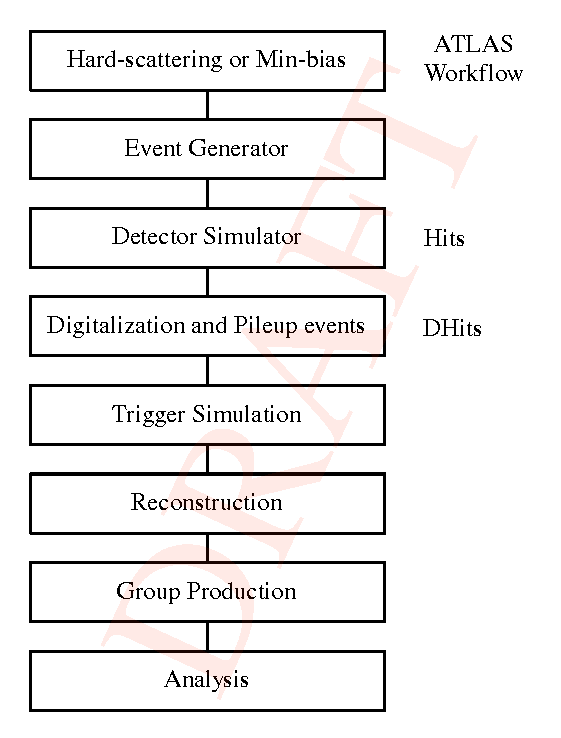
\includegraphics[width=\columnwidth]{figures/atlas_workflow.pdf}
  \caption{ATLAS Monte Carlo workflow.}
\label{fig:atlas_workflow}
\end{figure}

\subsubsection{High-level Description}

\paragraph{Fig.~\ref{fig:atlas_workflow} (1)} Multiple end-users (i.e.,
physicists) submit descriptions of ATLAS Monte Carlo Workflows to the JEDI
component of ATLAS middleware. JEDI supervises the execution of these workflows
through a set of eight predefined stages. Each stage requires a specific type of
input and returns a specific type of output. In this paper, we focus on the
third stage called ``Detector Simulator'': the only one, at the moment, executed
on the HPC resources of Titan.

\paragraph{Fig.~\ref{fig:atlas_workflow} (2)} JEDI submits/hands over events
to a PANDA Server. This server manages the execution of all the ATLAS workflows
and their stages, including the ATLAS Monte Carlo Workflow. In
Fig.~\ref{fig:atlas_workflow} we depicted only how the events of the third
stage are organized within PANDA Server. Tasks are container of jobs and each
job contains itself a set of events. Each task, each job in that task and all
the events of those jobs belongs to a specific user. This enables provenance
across the PanDA stack and isolating the management of the data of each task by
dedicated subsystems.

\paragraph{Fig.~\ref{fig:atlas_workflow} (3)} Sets of events belonging to
multiple tasks and jobs are pulled from the PANDA Server by one or more PANDA
Pilot. Currently, twenty PANDA Pilots are instantiated on four dedicated DSL
nodes of Titan. These pilots are responsible for the packaging of a set of
events into a PBS job script. Packaging is performed on the base of the
information gathered about the availability of backfill resources on Titan.
Depending on the amount of nodes available on Titan, a specific number of events
is packaged into the PBS script. It should be noted that the events packaged
into a PBS job can belong to different tasks and therefore users.

\paragraph{Fig.~\ref{fig:atlas_workflow} (4)} AthenaMP is used to perform the
simulation of the events within the ATLAS detector, one AthenaMP thread for each
core available on the Titan nodes. Currently, sixteen threads are used for each
node, each thread being able to simulate an average of 1 event every n??
minutes?/second? (see Fig.~\ref{distribution_amp_titan}). So far, no
description has been given of the flow of data required to simulate each event.


\subsubsection{Backfill - High-level Description}
PanDA pilots  interrogate TITAN's queue continuously in order to find unused resources. This is done by using \emph{showbf} which provides the current number of unused resources and the duration of their idle time.

If PanDA server queue is not empty, each PanDA pilot tries to have five PanDA jobs constantly running on the resources. Therefore, if unused resources are available, a PanDA pilot sends a new PanDA job on TITAN's queue every time that one of its PanDA jobs terminates its execution.

PanDA pilot implements a greedy approach i.e. it tries to obtain all the available resources with a single PAnDA job\aanote{Verify this}. The size of a PanDA job cannot exceed 300 nodes \aanote{why???}.

After the submission of a PanDA job,  the PanDA pilot waits up to five minutes. If the PanDA job does not start in such time interval then the PanDA pilot deletes the job from TITAN's queue and try to resubmit the job.

The resubmission might change the size of the PAnDA job is the number of available nodes is changed in the meantime.

No job is submitted to TITAN's queue If less than \emph{XXX} nodes are available or if they are not  available for at least 2 hours.

Once the PAnDA job is running on the nodes, it spawns an Athena-MP job per node. Each Athena-MP job runs 16 concurrent processes that are in charge for the simulation of 100 events. No Athena-MP job is submitted after another. Therefore, PanDA job terminates immediately after all the Athena-MP jobs completed their simulation.

Questions:
\begin{itemize}
\item Which is the component that performs showbf? The Pilot?
\item Do pilots compete for the same available nodes?
\item There is any restriction in terms of minimum wall-time or minimum number of nodes?
\item If yes, Are there restrictrions imposed by ORNL or by PanDA server?
\item Is PanDA job walltime fixed or flexible? Two hours?
\item Does the pilot initiate input staging as a consequence of available nodes? if yes, what happens if input data is not there?
\end{itemize}
